\documentclass[tikz,border=10pt]{standalone}
\usepackage{tikz}
\usetikzlibrary{positioning, arrows.meta}

\begin{document}

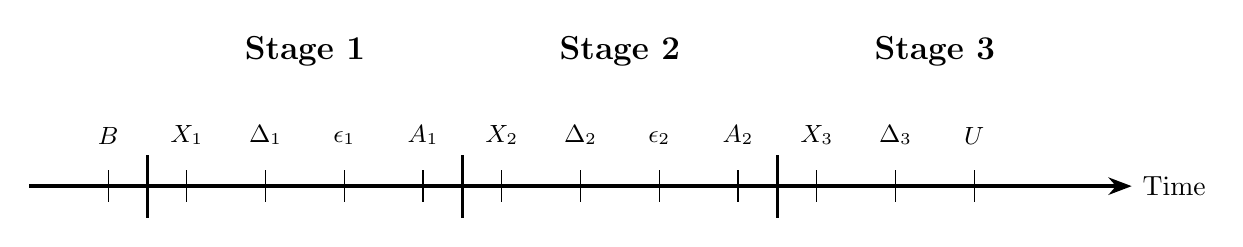
\begin{tikzpicture}[
    element/.style={
        font=\small,
        align=center
    }
]

% Main timeline
\draw[very thick, -Stealth] (0, 0) -- (14, 0) node[right] {Time};

% Section 1 elements - Small markers
\draw (1, -0.2) -- (1, 0.2);
\node[element, above=0.2cm] at (1, 0.2) {$B$};

% SECTION 1 - Large marker
\draw[very thick] (1.5, -0.4) -- (1.5, 0.4);
\node[above=1cm, font=\bfseries\large] at (3.5, 0.4) {Stage 1};

% Section 1 elements - Small markers
\draw (2, -0.2) -- (2, 0.2);
\node[element, above=0.2cm] at (2, 0.2) {$X_1$};

\draw (3, -0.2) -- (3, 0.2);
\node[element, above=0.2cm] at (3, 0.2) {$\Delta_1$};

\draw (4, -0.2) -- (4, 0.2);
\node[element, above=0.2cm] at (4, 0.2) {$\epsilon_1$};

\draw (5, -0.2) -- (5, 0.2);
\node[element, above=0.2cm] at (5, 0.2) {$A_1$};


% SECTION 2 - Large marker
\draw[very thick] (5.5, -0.4) -- (5.5, 0.4);
\node[above=1cm, font=\bfseries\large] at (7.5, 0.4) {Stage 2};

% Section 2 elements - Small markers
\draw (6, -0.2) -- (6, 0.2);
\node[element, above=0.2cm] at (6, 0.2) {$X_2$};

\draw (7, -0.2) -- (7, 0.2);
\node[element, above=0.2cm] at (7, 0.2) {$\Delta_2$};

\draw (8, -0.2) -- (8, 0.2);
\node[element, above=0.2cm] at (8, 0.2) {$\epsilon_2$};

\draw (9, -0.2) -- (9, 0.2);
\node[element, above=0.2cm] at (9, 0.2) {$A_2$};


% SECTION 3 - Large marker
\draw[very thick] (9.5, -0.4) -- (9.5, 0.4);
\node[above=1cm, font=\bfseries\large] at (11.5, 0.4) {Stage 3};

% Section 3 elements - Small markers
\draw (10, -0.2) -- (10, 0.2);
\node[element, above=0.2cm] at (10, 0.2) {$X_3$};

\draw (11, -0.2) -- (11, 0.2);
\node[element, above=0.2cm] at (11, 0.2) {$\Delta_3$};

\draw (12, -0.2) -- (12, 0.2);
\node[element, above=0.2cm] at (12, 0.2) {$U$};

\end{tikzpicture}

\end{document}
